
\section{Introduction}
\label{sec:intro}

Maintaining the performance of high-performance computing~(HPC) applications as
failures become more and more frequent is a major challenge that needs to be
addressed for next-generation extreme-scale systems.  Many recent studies have
demonstrated that hardware failures are expected to become ever more
common~\cite{Bergman08exascalecomputing}.  Increasing the scale of HPC systems
requires the aggregation of larger number of individual components.  More
components means more frequent failures.  Current systems use powerful
error-correcting codes~(ECC), e.g., chipkill-correct, to protect against DRAM
errors.  However, chipkill-correct (and other similar techniques) require the
activation of a large number of memory devices (four times more than
less-protective techniques like single error correct double error
detect~(SECDED))~\cite{Jian13}.  Activating more memory devices requires more
power for each memory access.  However, because of tightening power budgets on
next-generation systems~\cite{Bergman08exascalecomputing}, it is not yet clear
that chipkill-correct will continue to be viable.  Reduced device-feature sizes
also have the potential to result in more frequent failures.  Understanding the
implications of these trends requires that we have detailed knowledge of how
failures affect current leadership-class systems.

Recent works typically focus on uncorrectable errors, those errors that cause
applications to restart.  However, the impacts of the most common error of
large-scale systems, correctable errors, is typically overlooked. An analysis of
failures on recent leadership-class systems show that the correctable failure
rate is a factor \hl{ADD} more frequent than uncorrectable errors.  Correctable
errors are typically handled at a hardware level, and not reflected to the
application.  While the application continues to make progress in the presence
of these correctable errors and does not need to restart,the mechanism to
correct and log these errors have the potential to impact application
performance by delaying application computation.

\let\workinterval\relax
\let\ckpttime\relax
\let\txdelay\relax
\let\msgtime\relax
\let\minheight\relax
\newcommand{\workinterval}{1.25cm}
\newcommand{\ckpttime}{0.625cm}
\newcommand{\txdelay}{2.0mm}
\newcommand{\msgtime}{\workinterval+\txdelay}
\newcommand{\minheight}{0.5cm}
\usetikzlibrary{positioning}

\tikzstyle{position}=[fill=none,text=white,draw=none]
\tikzstyle{proc}=[fill=none,text=black,draw=none,shape=rectangle]
\tikzstyle{origtotal}=[fill=none,text=black,draw=black,shape=rectangle,
                       minimum width=3*\workinterval+2*\txdelay,
                       minimum height=\minheight]
\tikzstyle{coordtotal}=[fill=none,text=black,draw=black,shape=rectangle,
                        minimum width=3*\workinterval+\ckpttime+2*\txdelay,
                        minimum height=\minheight]
\tikzstyle{uncoordtotal}=[fill=none,text=black,draw=black,shape=rectangle,
                          minimum width=3*\workinterval+2*\ckpttime+2*\txdelay,
                          minimum height=\minheight]
\tikzstyle{ckpt}=[fill=black,text=white,draw=none,shape=rectangle,
                  minimum width=\ckpttime,minimum height=\minheight]
\tikzstyle{stall}=[fill=black!20,text=white,draw=black,shape=rectangle,
                   minimum height=\minheight]

\begin{figure*}[bt]
\centering{
\subfloat[without CE activity]{
\resizebox{0.25\textwidth}{!}{
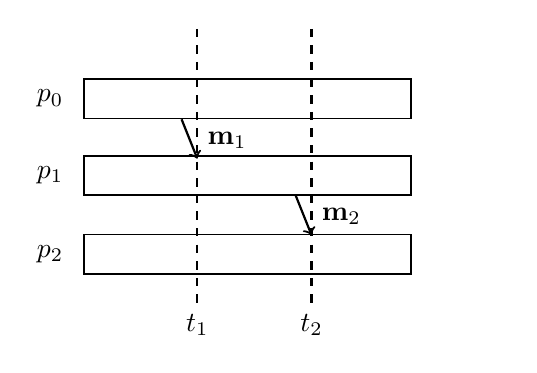
\begin{tikzpicture}[semithick]

\node [proc] (p0) {$p_0$};
\node [position, right= 0.125cm of p0, minimum width=3*\workinterval+2*\ckpttime+2*\txdelay] (n0) {};
\node [origtotal, right= 0.125cm of p0]  (v1) {};
\node [position, right= \msgtime of v1.north west ]  (v2) {};
\node [position, right= \msgtime of v2.west ]  (v4) {};

\node [proc, below = 5mm of p0] (p1) {$p_1$};
\node [origtotal, right= 0.125cm of p1]  (v5) {};
\node [position, right= \msgtime of v5.west ]  (v6) {};
\node [position, right= \workinterval of v6.south west ]  (v8) {};

\node [proc, below of=p1] (p2) {$p_2$};
\node [origtotal, right= 0.125cm of p2]  (v9) {};
\node [position, right= \msgtime of v9.west ]  (v10) {};
\node [position, right= \msgtime of v10.west ]  (v11) {};

\draw [->, thick] (v1.south west) ++(\workinterval,0) -- ++(\txdelay, -5.00mm) 
      node[above right] {$\mathbf{m}_1$};
\draw [->, thick] (v8.south west) -- ++(\txdelay, -5.00mm) node[above right] {$\mathbf{m}_2$};

\draw [thick, dashed] (v2.north west) ++(0.0cm, 5.0mm) -- (v10.south west) -- ++(0, -5.0mm) node[below] {$t_1$};
\draw [thick, dashed] (v4.north west) ++(0.0cm, 5.0mm) -- (v11.south west) -- ++(0, -5.0mm) node[below] {$t_2$};
\end{tikzpicture} 
}\label{subfig:no_ckpt}
}
%
%
%\subfigure[uncoordinated checkpointing]{
\subfloat[with local CE activity delays]{
\resizebox{0.25\textwidth}{!}{
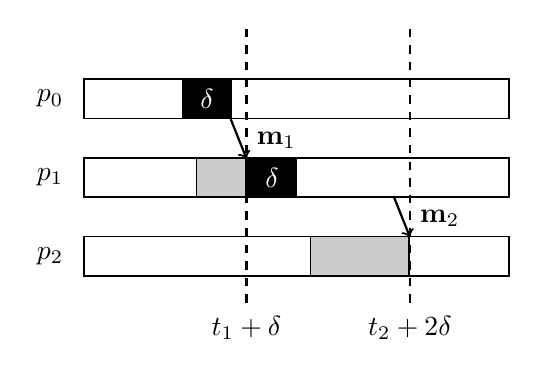
\begin{tikzpicture}[semithick]

\node [proc] (p0) {$p_0$};
\node [uncoordtotal, right= 0.125cm of p0]  (v1) {};
\node [position, right= \msgtime+\ckpttime of v1.north west ]  (v2) {};
\node [ckpt, right= \workinterval of v1.west ]  (v3) {$\delta$};
\node [position, right= \msgtime+\ckpttime of v2.west ]  (v4) {};

\node [proc, below of=p0] (p1) {$p_1$};
\node [uncoordtotal, right= 0.125cm of p1]  (v5) {};
\node [position, right= \msgtime+\ckpttime of v5.west ]  (v6) {};
\node [stall, minimum width=\ckpttime, left= 0.0cm of v6.west ]  (v7) {};
\node [ckpt, right= 0.00cm of v6.west ]  (v7) {$\delta$};
\node [position, right= \workinterval+\ckpttime of v6.south west ]  (v8) {};

\node [proc, below of=p1] (p2) {$p_2$};
\node [uncoordtotal, right= 0.125cm of p2]  (v9) {};
\node [position, right= \msgtime+\ckpttime of v9.west ]  (v10) {};
\node [position, right= \msgtime+\ckpttime of v10.west ]  (v11) {};
\node [stall, minimum width=2*\ckpttime, left= 0.00cm of v11.west ]  (v12) {};

\draw [->, thick] (v1.south west) ++(\workinterval+\ckpttime,0) -- ++(\txdelay, -5.00mm) 
      node[above right] {$\mathbf{m}_1$};
\draw [->, thick] (v8.south west) -- ++(2.0mm, -5.00mm) node[above right] {$\mathbf{m}_2$};

\draw [thick, dashed] (v2.north west) ++(0.0cm, 5.0mm) -- (v10.south west) -- ++(0, -5.0mm) node[below] {$t_1+\delta$};
\draw [thick, dashed] (v4.north west) ++(0.0cm, 5.0mm) -- (v11.south west) -- ++(0, -5.0mm) node[below] {$t_2+2\delta$};
\end{tikzpicture} 
}\label{subfig:uncoord_ckpt}
}
}
\caption{
        Example of how delays introduced by local correctable error (CE)
        activities may propagate along application communication dependencies.
        The processes $p_1$, $p_2$, and $p_3$ exchange two messages $m_1$ and
        $m_2$ in each of the three scenarios. The black regions marked with a
        white $\delta$ denote the execution of CE mitigation activities.  The
        grey regions denote periods in which the execution of a process is
        stalled due to an unsatisfied communication dependency.
}\label{fig:propagation}
\end{figure*}

\label{fig:propagation}

In an effort to better understand the impacts from correctable errors, in this
paper we present in-depth analyses that reveal how the interplay between
application and correctable protocol activities affect performance.  We
anticipate that this interplay will become increasingly more important as node
counts and memory volumes increase dramatically on future extreme-scale systems.
Additionally, smaller feature sizes, manufacturing variances, hardware aging
effects, and sub-threshold logic have the potential to further increase the
correctable error rates.  More specifically, using a wide array of application,
we demonstrate that the overheads of correctable errors can have a significant
impact on overall application performance.  These local correctable errors
introduce overheads that can amplified or absorbed globally by an application
depending on an application's communication activities.  We use profiles of
these communication activities as well as microbenchmark studies to more
precisely attribute each application's performance to its communication
operations.

The possibly of correctable error activities inducing delays amongst application
processes, including those that do not directly communicate, is analogous to
the manner in which operating system noise (or \emph{jitter}) can affect HPC
applications~\cite{Hoefler:2010:Characterizing, Ferreira:08:characterizing}.
\Cref{fig:propagation} illustrates this phenomenon.  \Cref{subfig:no_ckpt} shows
a simple application running across three processes ($p_0$, $p_1$, and $p_2$)
with no delays due to CE.  These three processes exchange two messages,
$\mathbf{m}_1$ and $\mathbf{m}_2$.  We assume here that these messages represent
strict dependencies: any delay in the arrival of a message requires the
recipient to stall until the message is received. \Cref{subfig:uncoord_ckpt}
illustrates the potential impacts due to local CE mitigation activity.  If $p_0$
receives a CE at the instant before it would have otherwise sent $\mathbf{m}_1$,
then $p_1$ is forced to wait (the waiting period is shown in grey) until the
message arrives.  If $p_1$ subsequently receives a CE before sending
$\mathbf{m}_2$, then $p_2$ is forced to wait.  Part of the time that $p_2$
spends waiting is due to a delay that was originated by $p_0$, which it does not
communicate with.  The key point is that delays due to correctable errors can
propagate based on communication dependencies in the application.

Based on the studies presented in this paper, we make the following
contributions:

\begin{itemize}

\item we demonstrate the impacts of the logging and tracking activities due to correctable
errors, and how those activities can changes based on platform configuration \S{?};
\item we analyze the potential impacts of this correctable errors on application
performance and how these impacts many change with increased errors rate \S\S{?};
\item we show how an application's scale and communication pattern can dictate
whether local overheads due to correctables are amplifies or absorbed by other
processes \S\S{?}; and
\item we show the interplay between the correctable error rate and the duration
of each mitigation activity, providing prescriptive advice on how best to reduce
overheads due to these common errors on leadership-class platforms \S{?}.

\end{itemize}

Overall, this work provides critical analysis and insight into the overheads of
common correctable errors and provides practical advice to users and systems
administrators in an effort to fine-tune performance to application and system
characteristics.
